\documentclass[12pt]{article}

\usepackage{graphicx}
\usepackage{epstopdf}
\usepackage[spanish]{babel}
\selectlanguage{spanish}
%\usepackage[english]{babel}
\usepackage[utf8]{inputenc}
\usepackage{hyperref}
\usepackage[left=3cm,top=3cm,right=3cm,bottom= 2.5cm,nohead,nofoot]{geometry}
\usepackage{braket}
\usepackage{datenumber}
\usepackage{textcomp}
\usepackage{chemfig}%figuras Quimica
\usepackage[version=4]{mhchem}%nombres compuestos quimicos
%\newdate{date}{10}{05}{2013}
%\date{\displaydate{date}}

\begin{document}

\begin{center}
%\Huge
\LARGE
Optimizaci\'{o}n de Simulaciones por Din\'{a}mica molecular para el Estudio de Propiedades Biof\'{i}sicas de Estafiloxantina en Membranas de DMPG y DPPG.\\
\vspace{3mm}
\large
John Erick Cabrera Ramirez 

%\large
 C\'odigo: 201823444


\vspace{2mm}
\large
Director: Chad Leidy

\normalsize
\vspace{2mm}

\today
\end{center}


\normalsize
\tableofcontents
%\begin{abstract}
 %   \textit{Resumen}
 %   
%\end{abstract}
\newpage
\section{Introducci\'on}

\textit{Staphylococcus aureus} es una bacteria pat\'{o}gena, que causa enfermedades infecciosas, del tipo Gram positiva. De acuerdo a REF7, la bacteria se encuentra en la piel y en el aparato respiratorio sin producir enfermedades en condiciones normales, pero que puede causar infecciones nicosomiales o intrahospitalarias en el sistema respiratorio, en los tejidos blandos y en el torrente sangu\'ineo \cite{1HarpavatS.NissimS.LipppincottsMicrocards:MicrobiologyFlashCards2012.}; incluso puede causar infecciones en las junturas de las pr\'otesis formando biopel\'iculas,  ver \cite{Meylan2018}.\\

En la figura \ref{fig:sta} se muestra una microfotograf\'ia de \textit{Staphylococcus aureus} resistente a antibi\'oticos.\\

\begin{figure}[h]
\begin{center}
  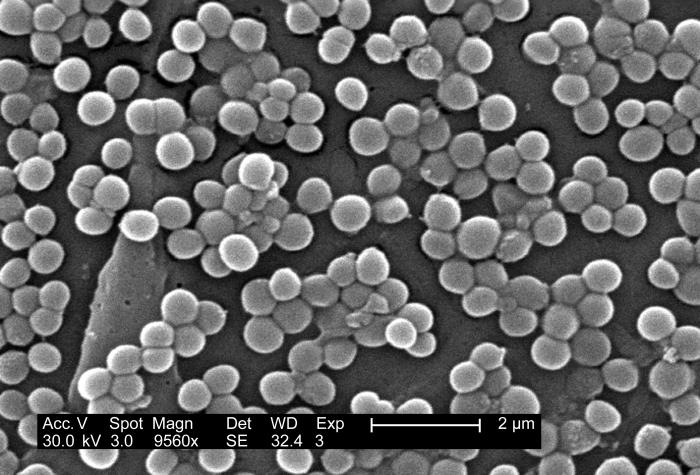
\includegraphics[scale=0.3]{saureus.jpg}
  \caption{Imagen  de \textit{Staphylococcus aureus} obtenida con un microscopio electr\'onico de barrido (SEM). Tomado de \cite{HaneyCar2005PublicAureus}.}
  \label{fig:sta}
\end{center}
\end{figure}

Desde el descubrimiento de \textit{S. aureus} como causante de una infecci\'on a una herida en 1881 \cite{Orent2006AMagazine}, se ha investigado su presencia en otras infecciones y se han utilizado antibi\'oticos como la penicilina, la meticilina y la vancomicina para controlar estas infecciones   \cite{1HarpavatS.NissimS.LipppincottsMicrocards:MicrobiologyFlashCards2012.}. Sin embargo, \textit{S. aureus} ha desarrollado resistencia a estos antibi\'oticos,  surgiendo la necesidad de buscar nuevos antibi\'oticos o incluso moléculas con un mecanismo de acción diferente. Algunas de estas nuevas moléculas son los péptidos antimicrobianos, estas se describen en la sección \ref{ss:anti}.\\

Se ha encontrado que la rigidez de la membrana es uno de los factores determinantes en la tolerancia a antibióticos. Para \textit{Staphylococcus aureus} la rigidez de la membrana interna, en adelante la bicapa lipídica, puede ser modulada con base en la concentración de los carotenoides y en particular de un triterpeno carotenoide llamado estafiloxantina \cite{Nagendra2011}.\\

La bicapa lipídica va a ser m\'as o menos r\'igida según su composición, lo cual implica corrimientos en la temperatura de transici\'on y cambios en la cooperatividad de la transici\'on de fase termotrópica. La estructura molecular de los fosfol\'ipidos presentes en la membrana hace que esta sea m\'as fluida cuando la estructura presenta mol\'eculas con m\'ultiples insaturaciones que inducen un incremento en espaciamiento, reduciendo la interacci\'on entre ellas. La membrana puede pasar de un estado s\'olido-ordenado (so) $L_{\beta}$ a un estado l\'iquido-desordenado (ld) $L_{\alpha}$ con un incremento de temperatura. En el caso de \textit{S. aureus} se ha descubierto que su membrana cambia el estado de rigidez de su membrana modulando la cantidad de estafiloxantinas presentes y la cantidad de cardiolipinas. \\
%En cuanto a la fluidez de la membrana de acuerdo a la temperatura, si se estudia una membrana compuesta \'unicamente por glicerofosfol\'ipidos, tal como se muestra en \cite{Heimburg}, esta presenta diferentes estados de acuerdo a su temperatura:  laminar l\'iquido cristalino, gel laminar, laminar ondulada, entre otras.\\

Debido a la importancia de la rigidez de la membrana lip\'idica en los procesos de defensa de la c\'elula e incluso para la b\'usqueda de nuevos antibi\'oticos, el objetivo principal es estudiar las propiedades biofísicas de los carotenoides de \textit{Staphyloccocus aureus} cuando están inmersos en membranas modelo de DPPG y DMPG, que simulan la membrana de \textit{Staphyloccocus aureus}.  Las membranas se estudian para los estados termotrópicos  $L_{\alpha}$ y  $L_{\beta}$ \\

Para estudiar las propiedades ópticas se usa la espectroscopía de fluorescencia. Mediante un fluorómetro, la espectroscopía de fluorescencia busca determinar el espectro de emisión y absorción de una molécula en solución, con lo cual podemos explorar la eficiencia cuántica, la cual provee información sobre que fracción de intensidad por segundo es emitida de forma radiactiva respecto a la intensidad por segundo incidente

\section{Estado del Arte}
\subsection{La membrana Bacteriana y sus compuestos presentes}\label{ss:mem}
Según el tipo de membrana que posean las bacterias, estás pueden clasificarse en dos grandes géneros: las bacterias Gram positivas y las bacterias Gram negativas. Las bacterias Gram positivas poseen una bicapa lipídica envuelta en una capa compuesta por unos polímeros de azúcares y aminoácidos llamados peptidoglicando, ver figura \ref{fig:mem} mientras que la membrana de una bacteria Gram negativa posee dos bicapas lipídicas. Ya que \textit{Staphylococcus aureus} es una bacteria Gram positiva se discutirá principalmente la composición de la membrana de las bacterias Gram Positivas.\\

\begin{figure}[h]
\begin{center}
  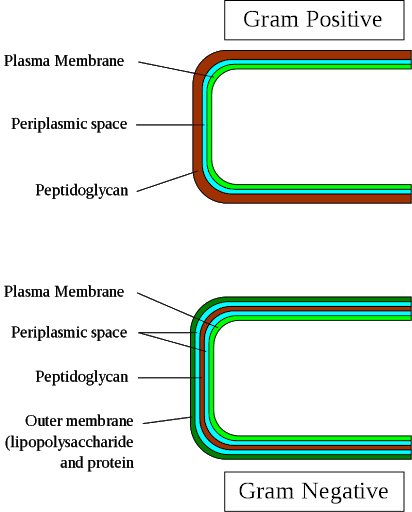
\includegraphics[scale=0.3]{grampos1.png}
    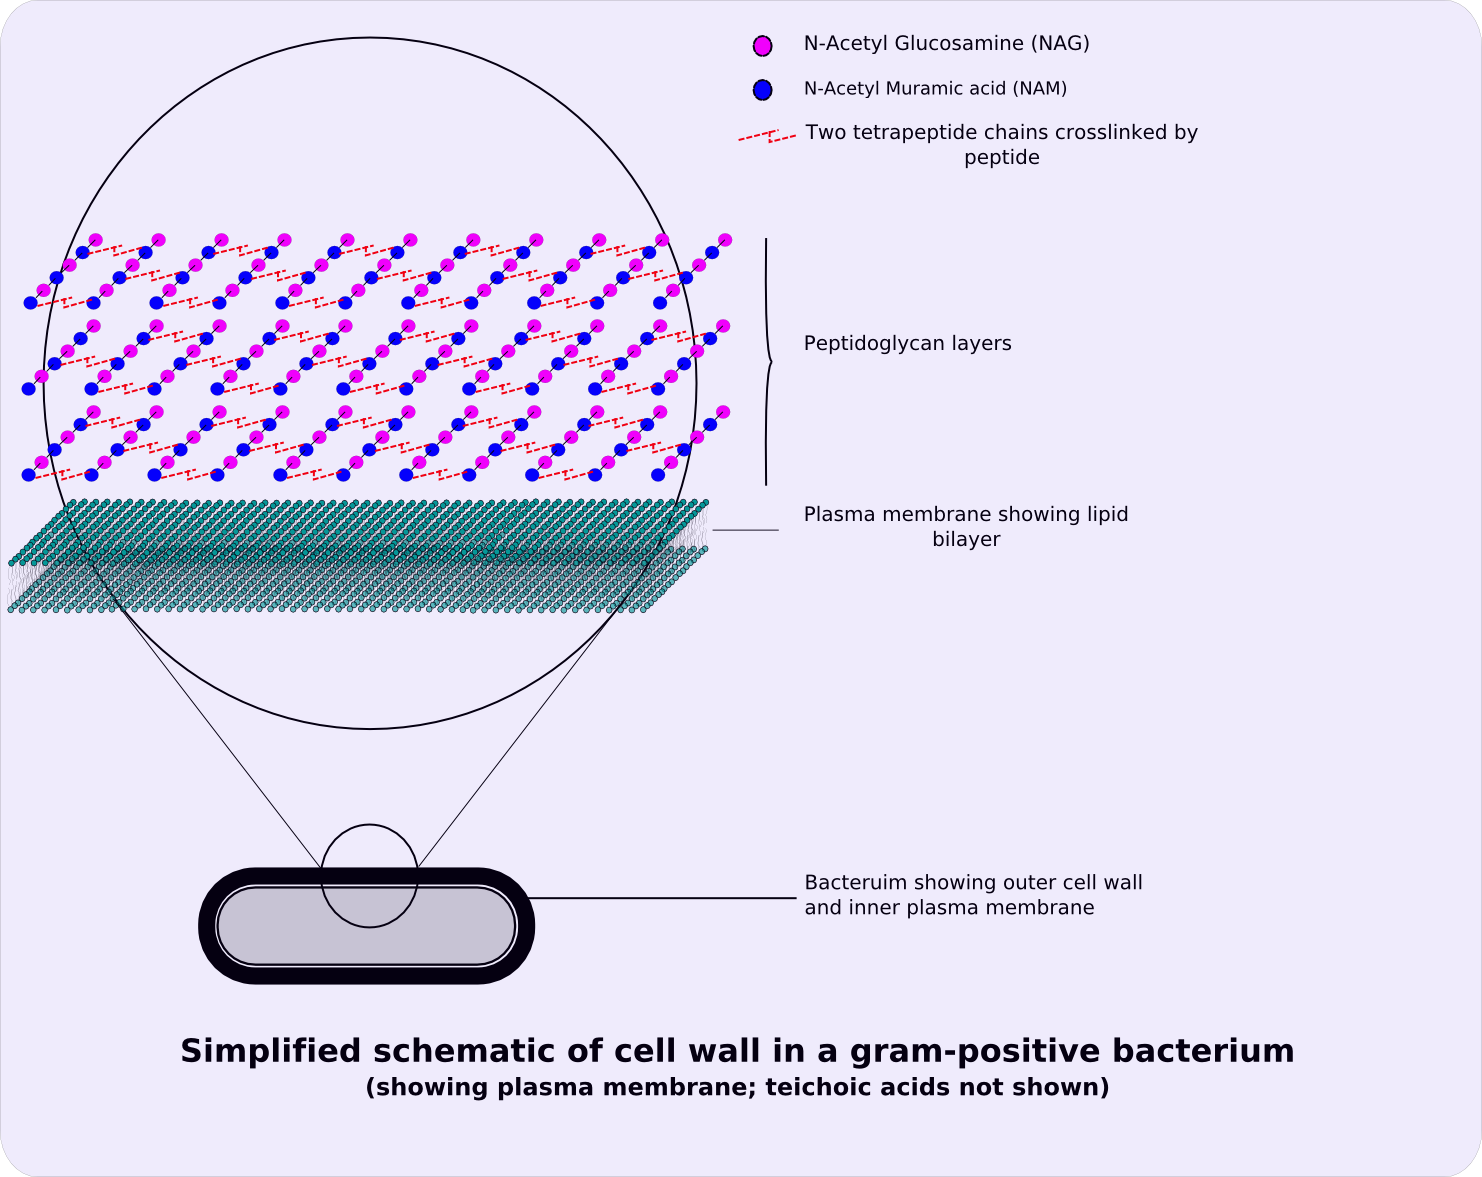
\includegraphics[scale=0.15]{grampos2.png}
  \caption{Imagen  de la membrana de una bacteria Gram positiva. Tomado de \cite{Nelson2011}.}
  \label{fig:mem}
\end{center}
\end{figure}
La bicapa lipídica es una membrana presente en todos las células y  que está compuesta mayoritariamente por lípidos. Los lípidos se acomodan de tal manera que el espesor de la membrana sea de dos lípidos. Todos los lípidos están compuestos por una o varias cadenas de ácidos grasos (cadenas hidrocarbonadas con carboxilo) unidas a diferentes sustituyentes los cuales pueden presentar carga o no a pH fisiológico. De acuerdo a los sustituyentes y al tipo de ácidos grasos cada lípido tiene un  nombre y unas propiedades como la carga y la polaridad.Los lípidos forman bicapas debido a la presencia del agua ya que al ser moléculas anfipáticas la parte hidrofílica del lípido interactúa con el agua mientras que la parte hidrofóbica no interactúa con esta. Estas interacciones hacen que sea más estable encontrar los lípidos inmersos en el agua formando agregados sin mezclarse con el agua. La interacci\'on lateral entre estas mol\'eculas se da trav\'es de fuerzas no covalentes lo que le confiere propiedades de cristal l\'iquido caracterizado por la capacidad de presentar transiciones de fase s\'olido-l\'iquido. \\

La bicapa lipídica de \textit{Staphylococcus aureus} esta compuesta principalmente por fosfatidilgliceroles (PG), cardiolipina (CL), lifosfoglicandos (LPG) y glicopeptidolípidos (GPL) \cite{Sohlenkamp2015BacterialPathways}. En la figura \ref{fig:DMPG} se muestra la fórmula estructural del Dimiristoilfosphatidilglicerol (DMPG), el cual es un lídido con el fosfatidilglicerol unido a dos miristoil (provenientes del ácido mirístico). Se observa que este lípido forma un espaciaminento entre las cadenas hidrocarbonadas más grande que la cabeza del lípido, esto hace que la presencia de DMPG disminuya la rigidez de la membrana plasmática.
\\

\begin{figure}[h]
\begin{center}
    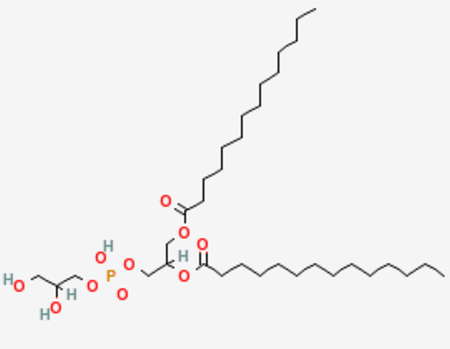
\includegraphics[scale=0.4]{DMPG.pdf}
  \caption{Fórmula estructural del Dimiristoilfosphatidilglicerol (DMPG). Tomada de \cite{CHEMDRUGDMPGDimyristoylphosphatidylglycerol}.}
  \label{fig:DMPG}
\end{center}
\end{figure}
Las membranas lipídicas además de tener lípidos contienen otros tipos de biomoléculas como los carotenoides, las proteínas y los glicolípidos que tienen relevancia fisiológica en la célula. Los carotenoides en particular pigmentan las células. En el caso de \textit{Staphylococcus aureus} se ha descubierto que los carotenoides juegan un papel importante en la integridad de la membrana celular y protegen a la bacteria frente a estrés oxidativo \cite{Nagendra2011}. La protección de los carotenoides en la membrana se ve reflejada por un aumento de su rigidez, de forma similar al papel que juega el colesterol en la membrana eucariótica. \\

Uno de los carotenoides más relevantes en \textit{Staphylococcus aureus} es la estafiloxantina la cual le da el nombre a la bacteria ya que le da un color aúreo. La estafiloxantina es un  triterpeno carotenoide en que posee dos cadenas hidrocarbonadas con insaturaciones conjugadas tipo trans, las dos cadenas están unidas a un azúcar mediante enlaces tipo eter, ver figura \ref{fig:stx}. Debido a los enlaces dobles conjugados de las cadenas hidrocarbonadas en la estafiloxantina, esta se convierte en un factor que aumenta el empaquetado de la bicapa lípidica, ya que disminuye la distancia entre los vecinos \cite{Heimburg}.\\

\begin{figure}[h]
\begin{center}
  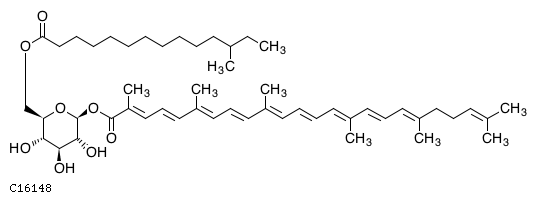
\includegraphics[scale=0.4]{staphyloxanthin.png}
  \caption{Fórmula estructural de la estafiloxantina. Tomada de \cite{KEGGC16148}.}
  \label{fig:stx}
\end{center}
\end{figure}
 Adem\'{a}s, estas insaturaciones conjugadas le da propiedades antioxidantes que protegen a la bacteria frente al estrés oxidativo del medio.
\subsection{Resistencia a tratamientos antibióticos de \textit{Staphylococcus aureus}}\label{ss:anti}
Desde que se ha descubierto que \textit{Staphylococcus aureus} es una bacteria patógena, se ha combatido con antibióticos como la penicilina pero a mediados del siglo XX \textit{Staphylococcus aureus} comenzó a presentar resistencia. Posteriormente se han aplicado otros antibióticos como la meticilina pero también ha presentado resistencia a este antibiótico. Otro antibiótico que se aplica como tratamiento a \textit{Staphylococcus aureus}  es la vancocimina. De ahí que surga la necesidad de buscar nuevos medicamentos que combatan \textit{S. aureus}.\\

Un p\'eptido antimicrobiano es un p\'eptido (es decir un olig\'omero de amino\'acidos) que hace parte de la respuesta inmune de los casi todos las formas de vida aunque también puede crearse sintéticamente. Los péptidos antimicrobianos se clasifican según la estructura secundaria que tienen: $\alpha$ h\'elices, $\beta$ plegados.   Los p\'eptidos antimicrobianos interact\'uan con la membrana de la bacteria produciendo orificios que causan p\'erdida de contenido y muerte celular.\\


\subsection{Transiciones de Fase en L\'ipidos}\label{ss:fase}
En soluci\'on con agua, los l\'ipidos tienden a formar agregados debido a  su car\'acter anfip\'atico. Para concentraciones mucho mayores a cierta concentraci\'on cr\'itica \cite{Heimburg}, los l\'ipidos tienden a formar bicapas. Las fases de estas bicapas se conocen como fases laminares y seg\'un su incremento en la temperatura se clasifican en:
\begin{itemize}
    \item \textit{Fase} $L_{c}$: Los l\'ipidos forman bicapas que presentan un orden en las tres dimensiones, es decir, las cabezas polares del l\'ipido presentan un patr\'on en forma de red mientras que las cadenas apolares est\'an ordenadas en configuraci\'on  trans.
    \item  \textit{Fase} $L_{\beta'}$: Esta es conocida como la fase gel. En esta los l\'ipidos se encuentran mayoriatariamente ordenados pero no todas cadenas hidrocarbonadas son trans. Se llama $\beta'$ porque algunos l\'ipidos presentan una inclinaci\'on respecto al plano de la normal, \cite{Heimburg}.
    \item  \textit{Fase} $P_{\beta '}$: Esta fase es una mezcla entre las fases de gel $L_{\beta '}$ y fluida $L_{\alpha}$. Se denomina as\'i porque la membrana presenta ondulaciones peri\'odicas.
      \item  \textit{Fase} $L_{\alpha}$: Esta es la fase l\'iquida o fluida de la membrana donde no hay un orden lateral de los grupos polares ni en las cadenas hidrocarbonadas.
\end{itemize}
Cuando ocurre una transici\'on de fase de primer orden, la presi\'on y la temperatura son aproximadamente constantes. El calor espec\'ifico a presi\'on constante se calcula mediante la relaci\'on:
\begin{equation}
    c_{p}=\left(\frac{\partial H}{\partial T}\right)_{P}
\end{equation}\label{eq:1}
Donde $H$ es la entalp\'ia del sistema, en este caso de la membrana bacteriana. Cuando ocurre la transici\'on de fase, hay un salto de la entalp\'ia. Cuando hay un salto en la entalp\'ia, el calor espec\'ifico $c_{p}$ presenta un pico, como una funci\'on tipo aguja.\\
Para liposomas con un solo l\'ipido se encuentran mediante m\'etodos de calorimetr\'ia las curvas de calor espec\'ifico mostradas en la figura \ref{fig:esp3}. Los tres compuestos son dimiristoil fosfatidilcolina ( por sus siglas en ingl\'es DMPC), dipalmitoilfosfatidilcolina ( por sus siglas en ingl\'es DPPC) y diasteroilfosfatidilcolina ( por sus siglas en ingl\'es DSPC).
\begin{figure}[h]
\begin{center}
  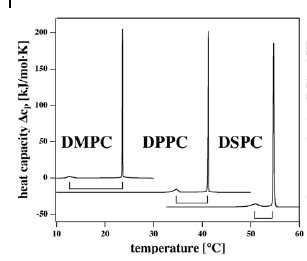
\includegraphics[scale=0.5]{cp.png}
  \caption{ Calor espec\'ifico en funci\'on de la temperatura para tres l\'ipidos diferentes. Los picos representan la transici\'on de fase cada uno.Tomado de \cite{Heimburg}}.
  \label{fig:esp3}
  \end{center}
\end{figure}
 Como la composici\'on de la bicapa fosfolip\'idica de \textit{S. aureus} no contiene \'unicamente el mismo tipo de fosfol\'ipidos, sino principalmente los que se han mencionado previamente, entonces no se espera obtener una transici\'on de fase con un salto perfecto, sino que tenga un ancho de banda tal como se muestra en la figura \ref{fig:ent2}, para m\'as detalles ver \cite{Ocampo2010TheAureus}.\\
\begin{figure}[h]
\begin{center}
  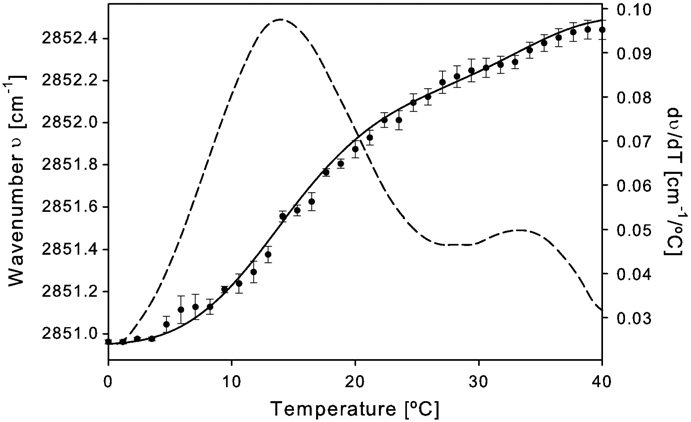
\includegraphics[scale=0.3]{transicion.png}
  \caption{ N\'umero de onda de la banda de CH$_{2}$ en funci\'on de la temperatura y su derivada para la membrana de \textit{S. aureus}. Imagen tomada de \cite{Ocampo2010TheAureus}.}
  \label{fig:ent2}
  \end{center}
\end{figure}
En la figura \ref{fig:ent2} cabe destacar que el n\'umero de onda es directamente proporcional a la energ\'ia de vibraci\'on de las mol\'eculas debido a la relaci\'on $E=h\nu$ con $\nu$ la frecuencia de vibraci\'on.\\
La gr\'afica \ref{fig:ent2} se obtuvo mediante la t\'ecnica de espectroscop\'ia de FITR variando la temperatura de la muestra.


\section{Objetivo General}

%Objetivo general del trabajo. Empieza con un verbo en infinitivo.
Estudiar las propiedades biof\'isicas de carotenoides de \textit{S. aureus} en la fases $L_\alpha$ y $L_\beta$ de membranas modelo de DMPG y DPPG a trav\'es del an\'alisis de espectroscop\'ia de fluorescencia.

\section{Objetivos Espec\'ificos}

%Objetivos espec\'ificos del trabajo. Empiezan con un verbo en infinitivo.

\begin{enumerate}
	\item 
	\item 
	\item 
	\item 
\end{enumerate}
\section{Metodolog\'ia}
\begin{itemize}
    \item \textbf{Objetivo 1} \textit{Aislar carotenoides totales de \textit{S.aureus} crecido en fase estacionaria.}\\
    
    \textbf{Extracción de carotenos apartir de \textit{S.aureus}} Para aislar los carotenoides de \textit{S.aureus} inicialmente se toma una colonia de la bacteria y se cultiva durante 48 horas en un agitador (overnight), el cultivo se coloca en la centrífuga obteniéndose en la parte baja un sedimento (pellet) y un supernadante (la parte superior). Luego se disuelven 50 $m$g del sedimento obtenido en la centrífuga en 1$m$L de metanol y se le añaden perlas de vidrio. La solución se mezcla en un vortex por 30s.  Posteriormente, se separan las células mediante una centrífuga que gira a 8500 rpm durante 15 min a 4\textdegree C. En la parte baja del frasco centrífugado se obtiene un sedimento y un supernadante que contiene carotenoides, fosfolípidos y proteínas. El supernadante que contiene los carotenos se lleva a otro frasco y se mezcla con 1.7M de \ce{NaCl} y acetato etílico con proporciones 3:1 V/V añadiendo primero el acetato etílico, al hacer esto se obtiene una separación de fases. Al centrifugar se obtiene en la fase superior una capa de acetato etílico la cual contiene carotenoides y lípidos, esta se pasa cuidadosamente a otro frasco mientras que a la fase inferior se le agrega 1$m$L de acetato etílico. Ambas fases orgánicas se combinan y se secan con \ce{Na_2SO_4} anhidro; la solución se decanta. El solvente con carotenoides se seca con \ce{N_2} obteniéndose un polvo. El polvo se disuelve en benceno y acetona en proporción 1:1 V/V, enfriándolo posteriormente a -20\textdegree C. Al hacer esto se precipitan los fosfolípidos y queda un supernadante con carotenoides. El supernadante con carotenoides se pasa a un frasco y se seca nuevamente con \ce{N_2}. Para realizar medidas de absorción se disuelve el secado en benceno. La cantidad de carotenoides se cuantifica mediante mediciones de absorción en el nanodrop entre 400$n$m y 550$n$m. Los carotenoides purificados se secan con benceno y se disuelven en cloroformo para incorporarlos a los liposomas modelo.
    
    \item \textbf{Objetivo 2} \textit{Generar vesículas unilamelares de DMPG y DPPG conteniendo carotenoides en proporciones de 5, 10,y 15 \% mol de carotenoides.}.\\
    
%Los vesículas unilamelares son generadas a partir de extractos de lípidos de \textit{Staphylococcus aureus}. Se realiza una extracción de lípidos para las fases de crecimiento exponencial y estacionaria. La extracción de lípidos es realizada por el procedimiento de Bligh and Dyer. En este procedimiento se toma la muestra bacterias y se pasa a una solución 1 a 2 V/V de cloroformo-etanol. La dilución se mezcla con un vortex y posteriormente se le añade 1 volumen de cloroformo, se mezcla. Luego, se añade agua destilada y se mezcla quedando una solución de cloroformo-etanol-agua de la cual se extraen los lípidos por filtros o por centrífuga, ver \cite{Perez-LopezVariationsProperties}.\\
\textbf{Preparación de las vesículas} Las vesículas se obtienen a partir de la mezcla de lípidos DMPG/carotenoides y DPPG/carotenoides. Para ello, se prepara un stock de lípidos y de los caratoneides  en cloroformo o cloroformo/metanol para los lípidos cargados. Luego se prepara la mezcla de lípidos para obtener 5, 10, 15\%mol de carotenos. Los solventes son secados utilizando vapor de  \ce{N_2} gaseoso, y los residuos son removidos por liofilización durante la noche (deshidratación de un material disminuyendo la temperatura y la presión). La capa de lipidos obtenida es hidratada con el buffer o solución amortiguadora (HEPES a 20mM y con 145 mM de \ce{NaCl}) obteniendo de esta forma vesiculas multilamelares. Para obtener las vesículas unilamelares, las multilamelares son extruidas por un filtro de membrana Whaltman \textregistered, \cite{Murphy2019WhatmanSciences}, por encima de la temperatura de transicion de los lípidos. Para las vesículas conteniendo DMPG se realiza a 40\textdegree C y para aquellas que contengan DPPG a 60\textdegree C.
\item \textbf{Objetivo 3} \textit{Estudio termotrópico de los espectros de emisión de carotenoides en membranas de DMPG y DPPG, determinando la eficiencia cuántica y los corrimientos en el espectro de emisi\'on en funci\'on de la concentración de carotenoides y el estado de fase $L_\alpha$ y $L_\beta$ de la membrana.}\\

\textbf{Medición de Espectros}
La influencia de los carotenoides en las membranas de DPPG y DMPG se hará utilizando el  espectrofotómetro contador de fotones ISS PC-1 acoplado a un control de temperatura, ver figura \ref{fig:fluo}. Este sistema permite la adquisición de los espectros de fluorescencia en función de la temperatura.
Según la intensidad de fluorescencia de la muestra, se colocan en el monocromador rendijas con ancho 0.5mm, 1mm o 2mm los cuales dejan pasar un ancho de banda de 2, 4 u 8 nm.\\
\begin{figure}[h]
\centering
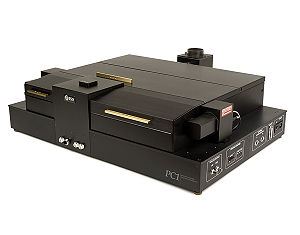
\includegraphics[scale=0.6]{300px-Spectrofluorimeter.jpg}
\caption{Fotografía del espectrofluorímetroa utilizar. Tomado de \cite{Suesca2019UAEquipment}.}
\label{fig:fluo}
\end{figure}

La muestra se prepara agregando 100$\mu$L de las vesíulas unilamelares disueltas en 1400$\mu$L de buffer (HEPES a 20mM y con 145 mM de \ce{NaCl}) en una cubeta, donde la mezcla se mantiene homogénea mediante un agitador magnético. Para cada muestra se determinan las rejillas adecuadas dependiendo de la intensidad de fluorescencia, esto se hace tomando una medida inicial del espectro. Un vez seleccionadas las rejillas, se realiza la toma de espectros de emisión y absorción para cada temperatura entre 10\textdegree C y 55\textdegree C de tal manera que se pueda pasar por la transición de fase termotrópica de las membranas. Los espectros son guardados mediante el software de adquisición de datos del espectrofotómetro. Una vez obtenidos los espectros, se determina el número de onda
para la máxima potencia radiada tanto de los espectros de absorción como de emisión, luego con cada valor se calcula un cuanto de energía $E=h\nu$ y con esto se halla la eficiencia cuántica, ecuación (2).
\item \textbf{Objetivo 4}\textit{Estudio de la anisotrop\'ia del espectro de emisi\'on de los carotenoides en membranas de DMPG y DPPG en las fases $L_\alpha$ y $L_\beta$ para determinar si existe una alineaci\'on preferencial de los carotenoides dentro de la membrana.}\\

\textbf{Anisotropía} Se realizan 6 mediciones en el espectrofluorómetro para membranas con DMPG y DPPG cada una a 5\%mol, 10\%mol y 15\%mol de carotenoides. Las mediciones se realizan usando el método de formato-L y en el estado estacionario (independiente del tiempo). Para realizar las medidas en el formato-L, el espectrofluorómetro tiene dos polarizadores UV grade Glan-Thompson, uno ubicado en el camino óptico de la fuente: polarizador de excitación y otro ubicado en el camino óptico del haz fluorescente: polarizador de emisión. El haz monocromático incidente pasa un polarizador vertical, luego llega a la muestra y de la muestra sale la radiación fluorescente. La radiación fluorescente pasa por un polarizador llamado polarizador de emisión ubicado a 90\textdegree de la dirección del haz incidente ver figura \ref{fig:aniso}, \cite{Lakowicz2006}.\\

Para realizar las mediciones inicialmente se configuran los polarizadores uno a 90\textdegree y el otro a 0\textdegree, luego se realiza el mismo procedimiento con los dos polarizadores alineados. Se configura el ancho de banda de la fuente de excitación a un ancho de banda de 2, 4 u 8 nm, tomando un ancho de rejilla de 0.5mm, 1mm o 2mm respectivamente.Inicialmente se realizan mediciones de prueba para un haz monocromático incidente entre 450$n$m y 490$n$m (color azul) y el haz de emisión se monitorea entre 560 y 590 $n$m (amarillo). La idea de esto es concocer como es el corrimiento de Stokes de los carotenoides en la membrana. Ya conociendo las longitudes de onda de los haces monocromáticos, se realizan mediciones del espectro de fluorescencia variando la temperatura entre  10\textdegree C y 55\textdegree C de tal manera que se pueda pasar por la transición de fase de las membranas.\\
\begin{figure}[h]
\centering
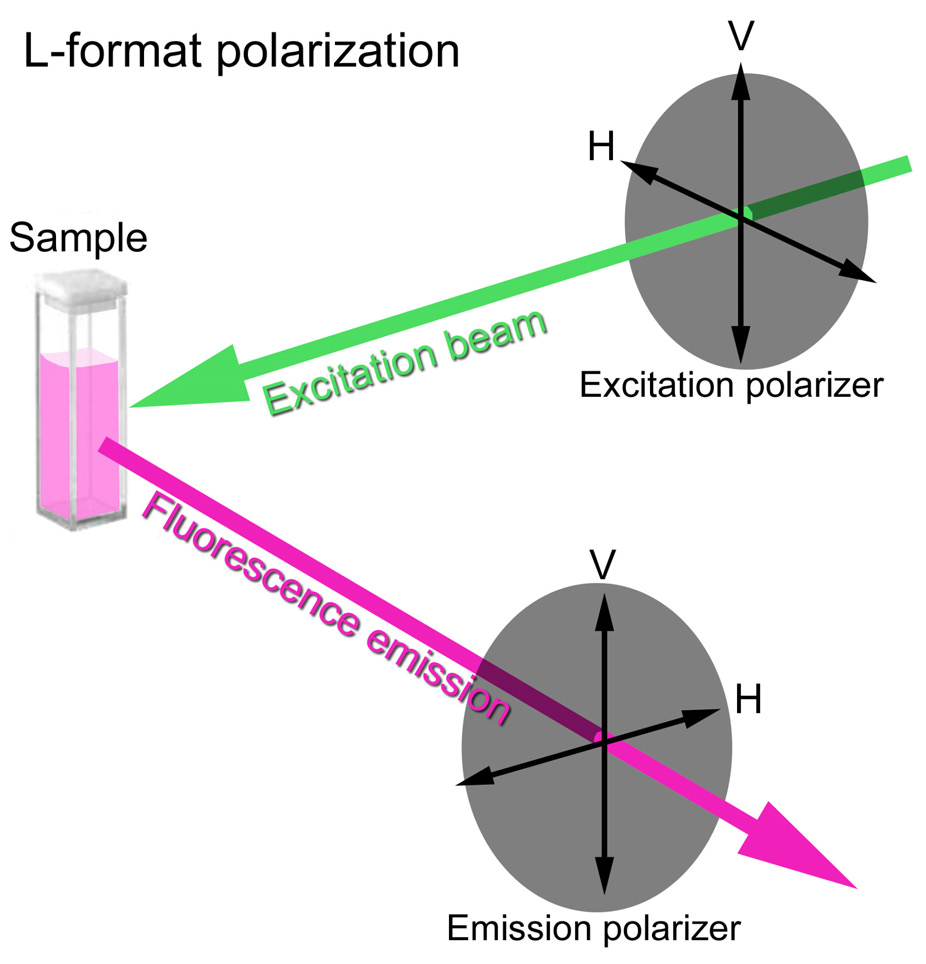
\includegraphics[scale=0.15]{aniso.png}
\caption{Medición de anisotropía en el formato L. Tomado de \cite{Lakowicz2006}.}
\label{fig:aniso}
\end{figure}
\end{itemize}

%Exponer DETALLADAMENTE la metodolog\'ia que se usar\'a en la Monograf\'ia. 

%Monograf\'ia te\'orica o computacional: ¿C\'omo se har\'an los c\'alculos te\'oricos? ¿C\'omo se har\'an las simulaciones? ¿Qu\'e requerimientos computacionales se necesitan? ¿Qu\'e espacios f\'isicos o virtuales se van a utilizar?

%Monograf\'ia experimental: Recordar que para ser aprobada, los aparatos e insumos experimentales que se usar\'an en la Monograf\'ia deben estar previamente disponibles en la Universidad, o garantizar su disponibilidad para el tiempo en el que se realizar\'a la misma. ¿Qu\'e montajes experimentales se van a usar y que material se requiere? ¿En qu\'e espacio f\'isico se llevar\'an a cabo los experimentos? Si se usan aparatos externos, ¿qu\'e permisos se necesitan? Si hay que realizar pagos a terceros, ¿c\'omo se financiar\'a esto?

\section{Cronograma}

\begin{table}[htb]
	\begin{tabular}{|c|cccccccc| }
	\hline
	Tareas $\backslash$ Semanas & 2 & 4 & 6 & 8 & 10 & 12 & 14 & 16\\
	\hline
	1 & X & X & X  &  X &   &   & &  \\
	2 &   &  & &  & X & X &X  & \\
	3 &   &   &  &  &   &   & & X\\
	4 &  &  &  &  &  &  & & \\
	\hline
	\end{tabular}
\end{table}
\begin{table}[htb]
	\begin{tabular}{|c|cccccccc| }
	\hline
	Tareas $\backslash$ Semanas & 18 & 20 & 22 & 24 & 26 & 28 & 30 & 32\\
	\hline
	1 &  &  &   &   &   &X  &X & X  \\
	2 &   &  &  &  & & X &  X &X\\
	3 & X  &X   & &  &   &  X &X & X\\
	4 &  &  & X & X & X &  X&X  &X \\
	\hline
	\end{tabular}
\end{table}
\vspace{1mm}

\section{Personas Conocedoras del Tema}

%Nombres de por lo menos 3 profesores que conozcan del tema. Uno de ellos debe ser profesor de planta de la Universidad de los Andes.

\begin{itemize}
\item	Jesus Perez Gil (Universidad Complutense de Madrid)\\
\href{mailto:jperezgi@ucm.es}{jperezgi@ucm.es}\\
\href{http://www.bbm1.ucm.es/biomil/}{http://www.bbm1.ucm.es/biomil/}
\item Marcela Manrique (Universidad de Antioquia)\\
\href{mailto:marcela.manrique@udea.edu.co}{marcela.manrique@udea.edu.co}
\item Luis Bagatolli  (MEMPHYS Universidad de Copenhagen)\\
\href{mailto:lbagatolli@immf.uncor.edu}{lbagatolli@immf.uncor.edu}\\
\href{http://memphys.dk/people/luis/index.html}{http://memphys.dk/people/luis/index.html}
\item Antonio Manu Forero Shelton (Universidad de los Andes)\\
\href{mailto:anforero@uniandes.edu.co}{anforero@uniandes.edu.co}
\end{itemize}
\bibliographystyle{ieeetr}
\bibliography{references}

%\begin{thebibliography}{10}

%\bibitem{Jerry} J. Banks. \textit{Discrete-Event System Simulation}. Fourth Edition. Prentice Hall International Series in Industrial and Systems Engineering, pg 86 - 116 y 219 - 235, (2005).

%\bibitem{Bronner} P. Bronner, A. Strunz, C. Silberhorn \& J.P. Meyn. European Journal of Physics, \textbf{30}, 1189-1200, (2009).

%\bibitem{LabInt} P. D\'iaz \& N. Barbosa: \textit{Obtenci\'on de n\'umeros aleatorios}. Informe final del curso Laboratorio Intermedio. Universidad de Los Andes, Bogot\'a, Colombia, (2012).

%\bibitem{Stefannov} A. Stefanov , N. Gisin , O. Guinnard , L. Guinnard \& H. Zbinden. Journal of Modern Optics, \textbf{47}:4, 595-598, (2000).

%\end{thebibliography}

\section*{Firma del Director}
\vspace{1.5cm}


\end{document} 